\documentclass{article}

\usepackage{graphicx}
\usepackage{tikz}
\usepackage{tikzsymbols}
\usetikzlibrary{calc,patterns,shapes.geometric}
\pagestyle{empty}
\usepackage[margin=0pt]{geometry}
\geometry{papersize={14in,12in}}

\def\centerarc[#1](#2)(#3:#4:#5){\draw[#1] ($(#2)+({#5*cos(#3)},{#5*sin(#3)})$) arc (#3:#4:#5);}

\begin{document}
	\begin{figure}
		\centering
		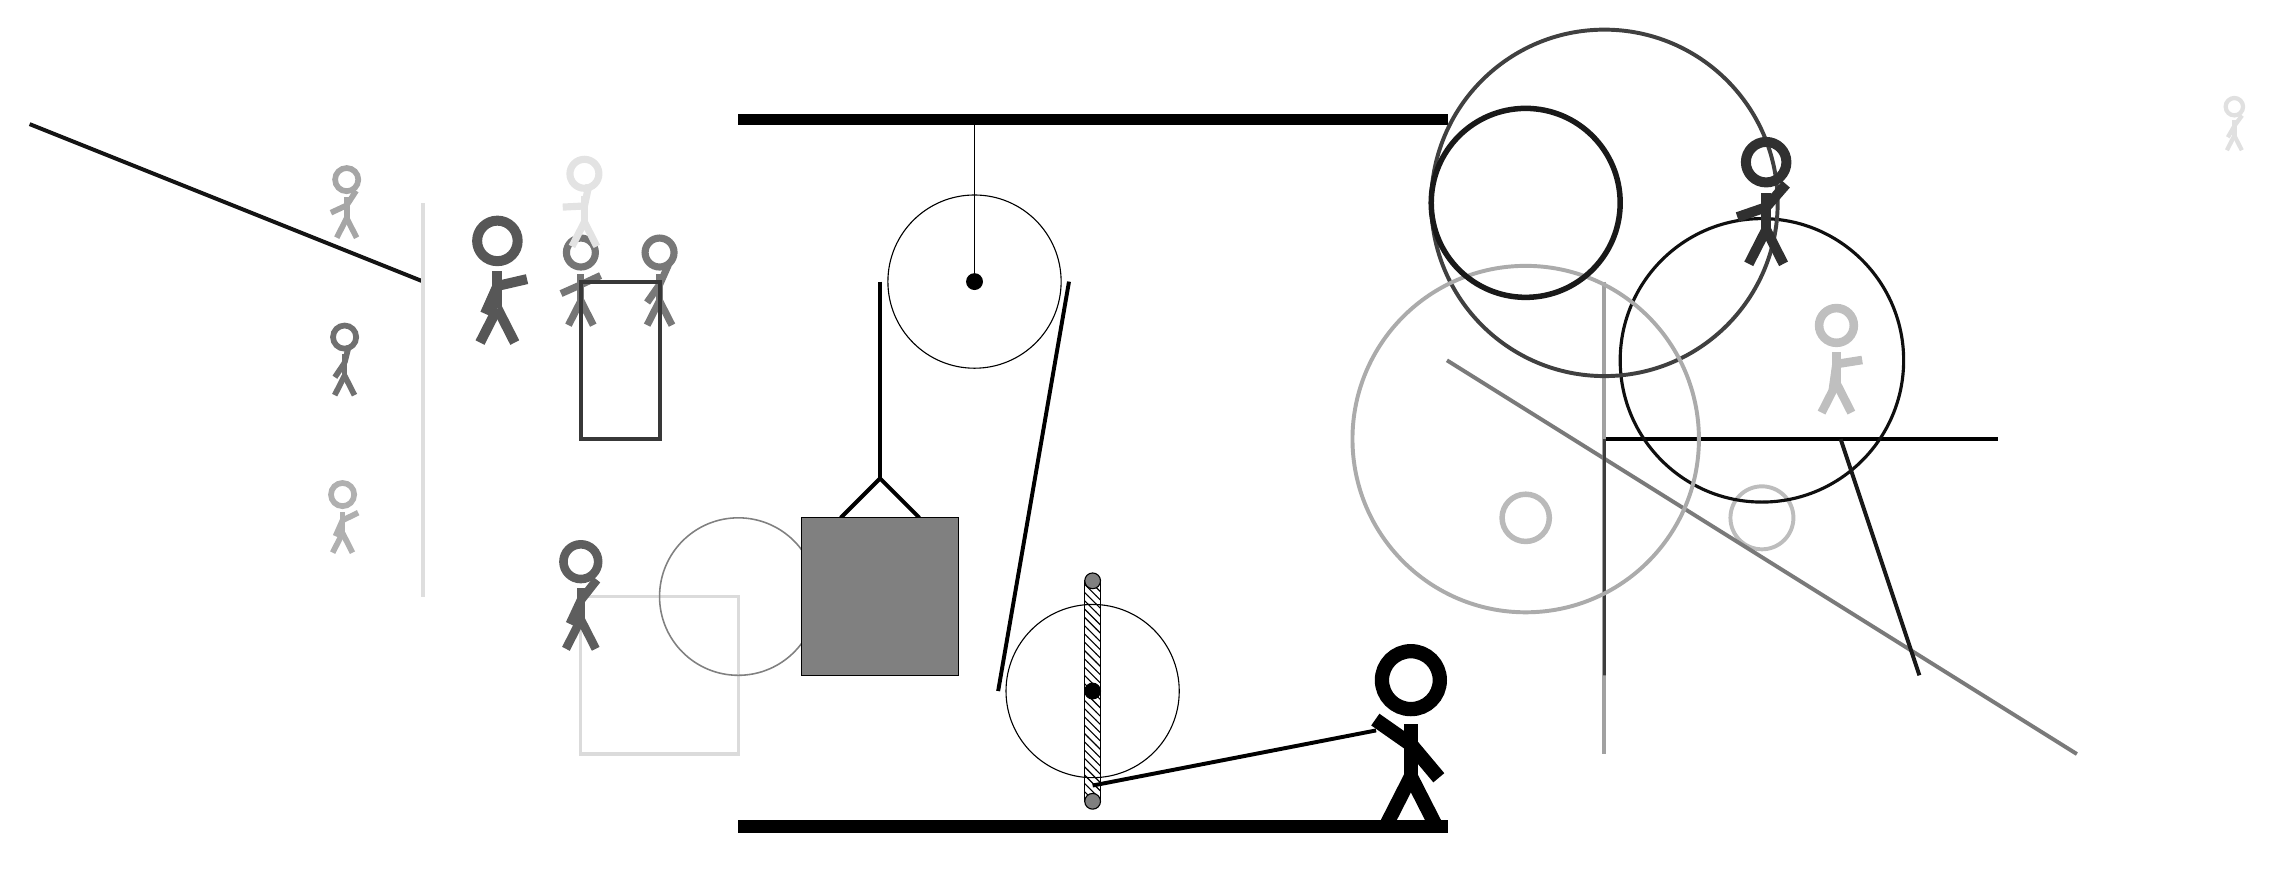
\begin{tikzpicture}
			%%%%% START %%%%%
			
			\draw[fill=black] (-2, 9) rectangle (7, 9.125);
			
			\draw[line width=0.5mm, color=black!100](9, 5) -- (14, 5);
			
			\draw [line width=0.5mm, color=black!26](11, 4) circle (0.4);
			\node[line width=0.3mm, color=black!54] at (-4, 7) {\Strichmaxerl[5][24][25]};
			\draw[line width=0.5mm, color=black!37](9, 7) -- (9, 1);
			\draw[line width=0.4mm, color=black!14] (-4, 1) rectangle (-2, 3);
			\node[line width=0.4mm, color=black!12] at (17, 9) {\Strichmaxerl[3][60][54]};
			
			\draw [line width=0.2mm, color=black!50](-2, 3) circle (1.0);
			\draw[line width=0.5mm, color=black!52](7, 6) -- (15, 1);
			\node[line width=0.3mm, color=black!31] at (-7, 4) {\Strichmaxerl[4][66][26]};
			\draw [line width=0.4mm, color=black!94](11, 6) circle (1.8);
			\draw [line width=0.5mm, color=black!75](9, 8) circle (2.2);
			\node[line width=0.6mm, color=black!25] at (12, 6) {\Strichmaxerl[6][82][9]};
			\draw[line width=0.3mm, color=black!76] (9, 5) rectangle (9, 2);
			\draw [line width=0.5mm, color=black!33](8, 5) circle (2.2);
			\node[line width=0.2mm, color=black!35] at (-7, 8) {\Strichmaxerl[4][25][57]};
			\node[line width=0.5mm, color=black!11] at (-4, 8) {\Strichmaxerl[5][3][78]};
			\draw[line width=0.5mm, color=black!92](-6, 7) -- (-11, 9);
			\node[line width=0.5mm, color=black!81] at (11, 8) {\Strichmaxerl[7][19][49]};
			\draw[line width=0.5mm, color=black!90](12, 5) -- (13, 2);
			\draw [line width=0.7mm, color=black!27](8, 4) circle (0.3);
			\node[line width=0.6mm, color=black!66] at (-5, 7) {\Strichmaxerl[7][66][13]};
			\node[line width=0.6mm, color=black!56] at (-7, 6) {\Strichmaxerl[4][56][76]};
			\node[line width=0.2mm, color=black!63] at (-4, 3) {\Strichmaxerl[6][65][52]};
			\draw[line width=0.5mm, color=black!13](-6, 3) -- (-6, 8);
			\draw [line width=0.7mm, color=black!90](8, 8) circle (1.2);
			
			\node[line width=0.2mm, color=black!53] at (-3, 7) {\Strichmaxerl[5][55][66]};
			
			\draw[line width=0.5mm, color=black!78] (-3, 5) rectangle (-4, 7);
			
			\draw (1, 7) circle (1.1);
			\draw[fill=black] (1, 7) circle (0.1);
			\draw (1, 9) -- (1, 7);
			
			\draw[fill=white](2.5, 1.8) circle (1.1);
			\draw[fill=black] (2.5, 1.8) circle (0.1);
			\draw[pattern=north west lines, pattern color=black] (2.4, 3.2) rectangle (2.6, 0.4);
			\draw[fill=black!50] (2.5, 3.2) circle (0.1);
			\draw[fill=black!50] (2.5, 0.4) circle (0.1);
			
			\draw[line width=0.5mm] (-0.7, 4.0) -- (-0.2, 4.5) -- (0.3, 4.0);
			\draw[fill=black!50] (-1.2, 4.0) rectangle (0.8, 2.0);
			
			\draw[line width=0.5mm] (-0.2, 7) -- (-0.2, 4.5);
			\centerarc[line width=0.5mm](1, 7)(0:180:1.2000000000000002);
			\draw[line width=0.5mm](2.2, 7) -- (1.3, 1.8);
			\centerarc[line width=0.5mm](2.5, 1.8)(180:270:1.2000000000000002);
			\draw[line width=0.5mm](2.5, 0.6) -- (6.1, 1.3);
			
			\node at (6.5, 1.2) {\Strichmaxerl[10][-35][-50]};
			
			\draw[fill=black] (-2, 0) rectangle (7, 0.15);
			
			%%%%% END %%%%%
		\end{tikzpicture}
	\end{figure}	
\end{document}